\section {Descripción general del producto}
	El producto que se desea fabricar es una mesa de billar, en particular una mesa de \emph{Pool con tapiz azul}.

Existen varios tipos de mesa de billar en función de la modalidad o tipo de juego y del tamaño de esta. A continuación se muestran algunos tipos de mesas de billar:

\begin{itemize}
\item {\bf Carambolas}
 Las mesas de carambolas no poseen agujeros. Puede ser clásica o innovadora, con el tapizado verde o  con el tapizado azul y el borde de madera.
\item {\bf Pool} 
Las mesas de pool tienen seis agujeros, cuatro en las esquinas y dos en la mitad de los dos lados más largos. Hay distintos tipos de mesas de \emph{Pool} en función del color del tapete y material del borde.
\item {\bf Snooker}
Las mesas de \emph{snooker} son similares a las mesas de \emph{Pool}. Pero son algo más grandes, con el tapiz más tupido y con las troneras más pequeñas y redondeadas. Suelen tener el tapizado verde y los bordes de madera
\end{itemize}

	  \begin{center}
    			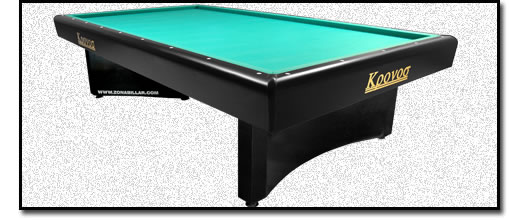
\includegraphics[width=0.4\textwidth]{PiramidCaram.jpg} \\
 \small { Mesa de Billar de Carambola  Clásica}
		\end{center}

La descripción general del producto a grandes rasgos es la siguiente: La mesa de billar es una mesa de madera en la que se apoya una losa de pizarra forrada de paño rodeada de bandas de material elástico y con seis agujeros y seis troneras. 
	
	\subsection {Utilidad y aplicaciones}
	La mesa de billar es usada para la práctica de un deporte llamado billar. Este deporte olímpico desde el 2004, tuvo sus inicios en la 
 antigua  Grecia y Egipto, pero es en la Europa del siglo XV cuando se empezó a tomar la forma del juego que se conoce en la actualidad. 

El billar consiste en impulsar un número variable de bolas con la ayuda de un taco, el cual lleva adosado en su extremo anterior una suela de cuero.
Con este movimiento debemos procurar introducir las bolas, de materiales sintéticos con cualidades elásticas similares a las del marfil, dentro de las troneras.
   
\section {Diseño del producto}
A continuación se va a mostrar la imagen de un diseño de una mesa de billar hecha con \emph{Blender}. Blender es un programa de diseño  multiplataforma, dedicado especialmente al modelado, animación y creación de gráficos tridimensionales.

  \begin{center}
 
\includegraphics[width=0.10\textwidth]{crystal_clear_app_blender.png} 
\\ \small {Logotipo de \emph{Blender}}
\end{center}

Esta imagen no se corresponde con la mesa de Billar a fabricar, pero puede servir para documentar algunas piezas de la mesa
y mostrar un ejemplo de un posible diseño de una mesa de Pool con un programa informático.

  \begin{center}


    			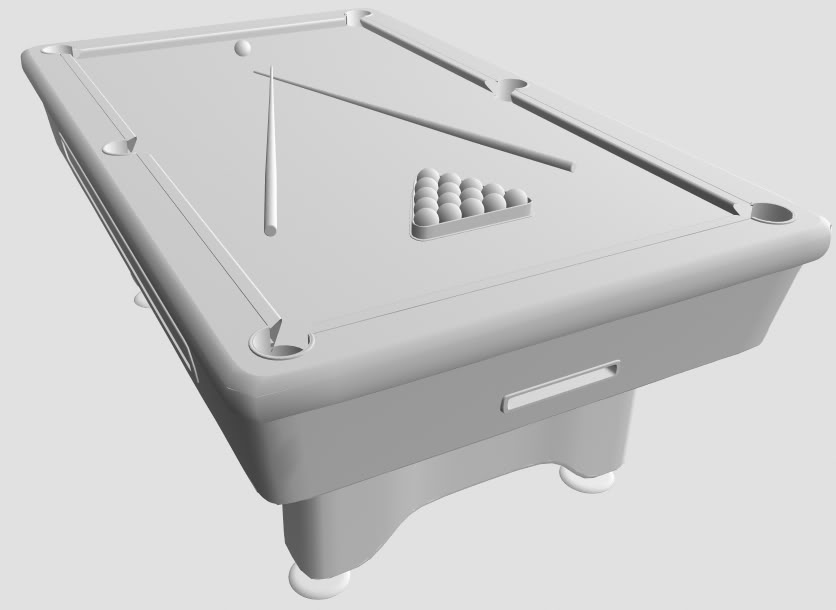
\includegraphics[width=0.40\textwidth]{prueba_billar.jpg} 
			\\ \small {Diseño realizado con \emph{Blender}}
		\end{center}

	\subsection {Definición técnica}
			\begin{enumerate}
			\item Las medidas de la mesa de billar pueden variar ligeramente siempre y cuando respetemos algunas medidas estándar. En este caso las medidas elegidas para la mesa son:
				\begin{itemize}      
				\item Medidas del campo de juego del billar: 200 x 100 cm.

				\item Medidas exteriores: 205 x 105 Altura: 80 cm
				\end{itemize}
				
			\item La superficie de la mesa es una la losa de pizarra 20 mm. Recubierta de un fieltro (lana y Poliamida) azul de 600 g.

			\item Los bordes del campo de juego en los que las bolas tienen que rebotar están compuestos por goma vulcanizada más lana.
			\end{enumerate}


	\subsection {Definición geométrica}
		    \begin{itemize}
		     \item La superficie del juego debe ser rectangular y poseer 6 agujeros por donde se introducirán las bolas de 5,715 cm (± 0,127 mm). Los agujeros estarán distribuidos como
			    muestra la siguiente figura.
		  \begin{center}
    			\includegraphics[width=0.25\textwidth]{billar.png} 
			\\ \small {Distribución de agujeros en una mesa de Pool.}
		\end{center}

		     \item Los bordes del campo (goma) están por todo el perímetro del campo salvo por donde hay agujeros y miden 3 cm de grosor.

		     \item Para la definición geométrica de cómo son las demás piezas  se adjunta vista general del producto, que explique mejor que apariencia tiene la mesas de billar
			  y sus diferentes elementos. 
		\begin{center}
    			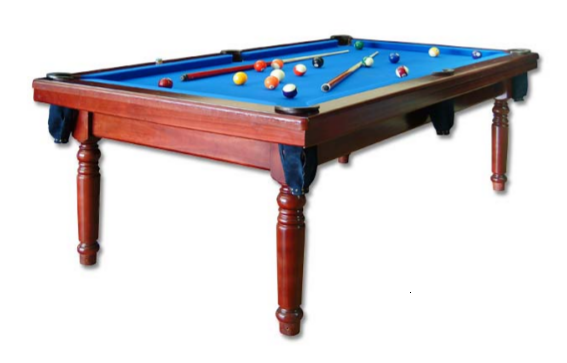
\includegraphics[width=0.5\textwidth]{donbillar.png}
     \\ \small {Mesa de Pool con elegante acabado clásico}
		\end{center}	
		    \end{itemize}
		    

	\subsection {Definición mecánica}
		    Cuando una bola cae a un agujero se pueden fabricar muchos y muy complejos mecanismos de recogida de la bola pero un mecanismo muy extendido,
		    fiable y muy empleado en las mesas de billar que residen en las viviendas, es poner unas troneras que guarden la bola una vez caída por el agujero hasta que queramos empezar
		    el juego de nuevo. Estas troneras o recipientes pueden ser de muchos materiales pero en nuestro caso serán de terciopelo azul  y lo suficientemente grandes como para quepan al menos cinco  bolas. 

\clearpage
\section {Fabricación del producto}

	\subsection {Proceso de fabricación detallado}
		A  continuación vamos a  ir detallando paso por paso cómo se fabrican una mesa de billar y sus diferentes piezas.
		
		\subsubsection {Preparar el tablero de pizarra}
			En primer lugar vamos a explicar cómo fabricar la pieza base de la mesa, el tablero o superficie de juego, hecho de pizarra. Este no tiene que ser necesariamente de pizarra pero es el mejor material, debido a  su resistencia y elasticidad.

 No todas las pizarras son igual de buenas para una mesa de billar, lo que hace que una pizarra sea buena y otra no es el contenido en cuarzo, cuanto menos tenga mejor será.

Para poder llegar hasta la pizarra solo se puede hacer combinando potentes motosierras con dinamita, para poder así obtener bloques gigantescos de pizarra.

	\begin{center}
	    		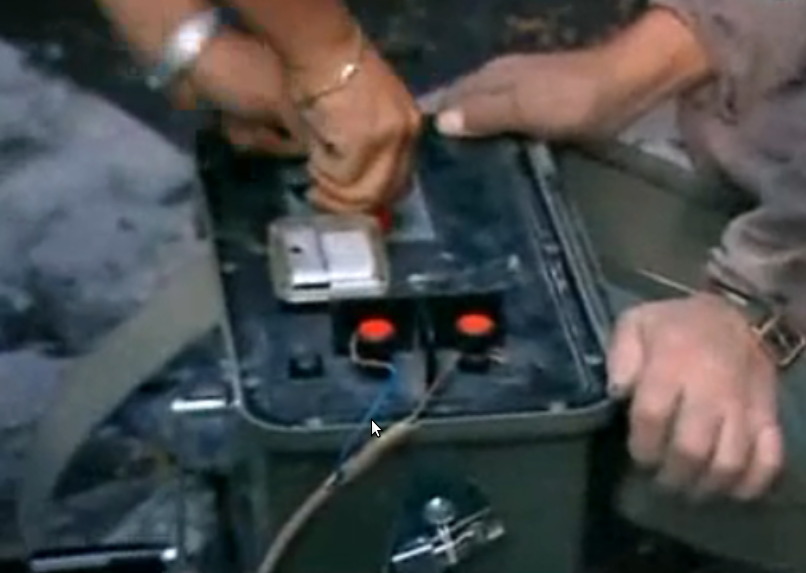
\includegraphics[width=0.4\textwidth]{Pantallazo-1.png}			
    \\ \small {Detonador de dinamita} \\[0.5cm]
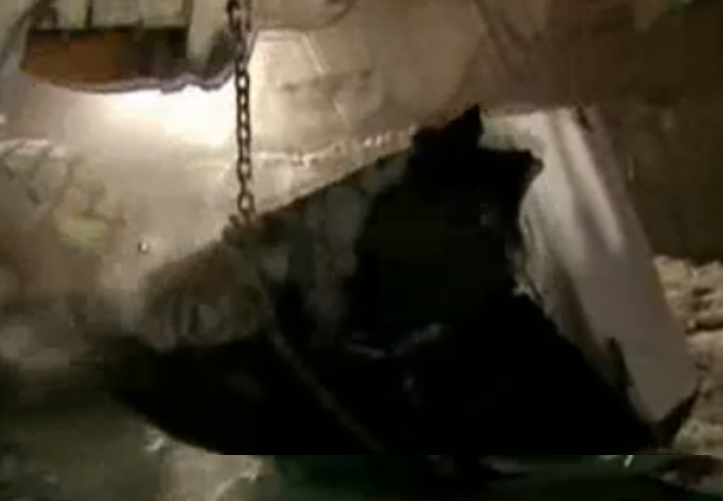
\includegraphics[width=0.4\textwidth]{Pantallazo-2.png} 
\\ \small {Excavadora trasportando bloque de pizarra}
	\end{center}

 Cuando tenemos el bloque de pizarra, este es trasportado a una marmolería donde se trasformará en la pieza que formará la mesa de billar.


Como el bloque de pizarra es enorme  no se puede partir  en trozos que sirvan para una mesa de billar, primero hay que cortar el bloque en losas que se puedan manejar. Para ello se utiliza una enorme sierra que corta la pizarra en gruesas lonchas. 

Para evitar que la pizarra se quiebre hay que cortarla muy despacio y refrigerar con agua continuamente las hojas de las sierras. 
	\begin{center}
	    		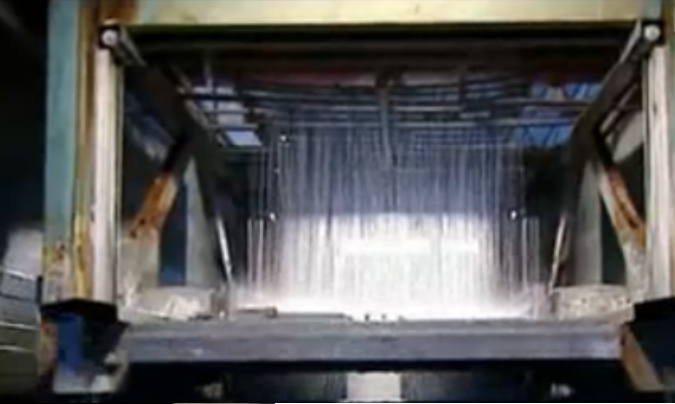
\includegraphics[width=0.4\textwidth]{Pantallazo-3.png}
\\ \small {Máquina encargada de cortar la pizarra}
	\end{center}


Como la pizarra esta formada por una serie de capas asentadas una sobre otra, los cortes tienen que ser hechos  a lo largo de esas lineas de división.
  La estructura rígida  de la pizarra hace que si se corta en la dirección correcta producirá losas finas de un grosor uniforme, para ello se emplea un cincel y un martillo para separar las losas de pizarra de forma manual.
	\begin{center}
	    		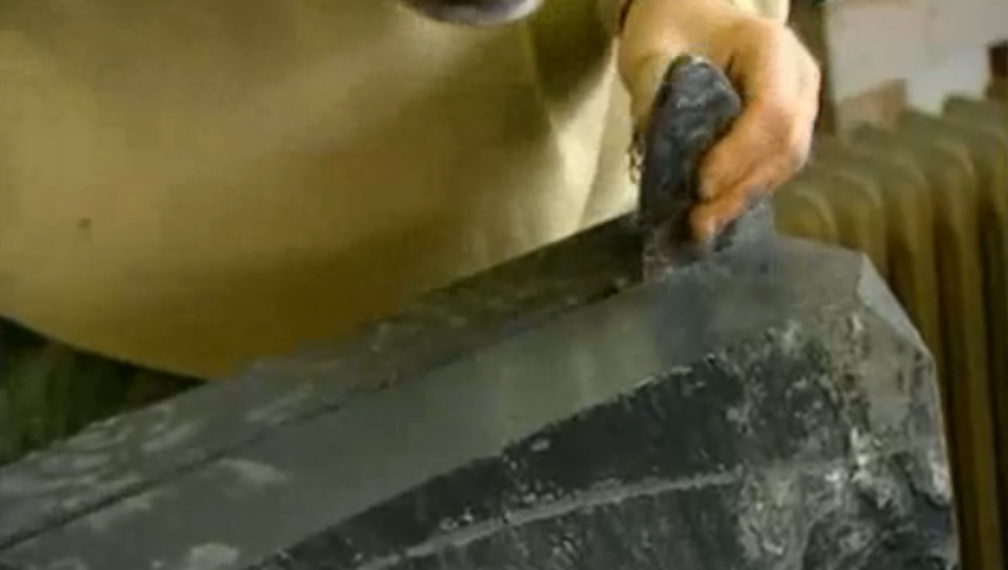
\includegraphics[width=0.4\textwidth]{Pantallazo-5.png}
			\\ \small {Separación manual de las losas de pizarra}
	\end{center}

Cuando ya tenemos la losa de pizarra, la cortamos con las dimensiones deseadas (2 m x 1 m) ayudándonos de unas radiales. 
\begin{center}
	    		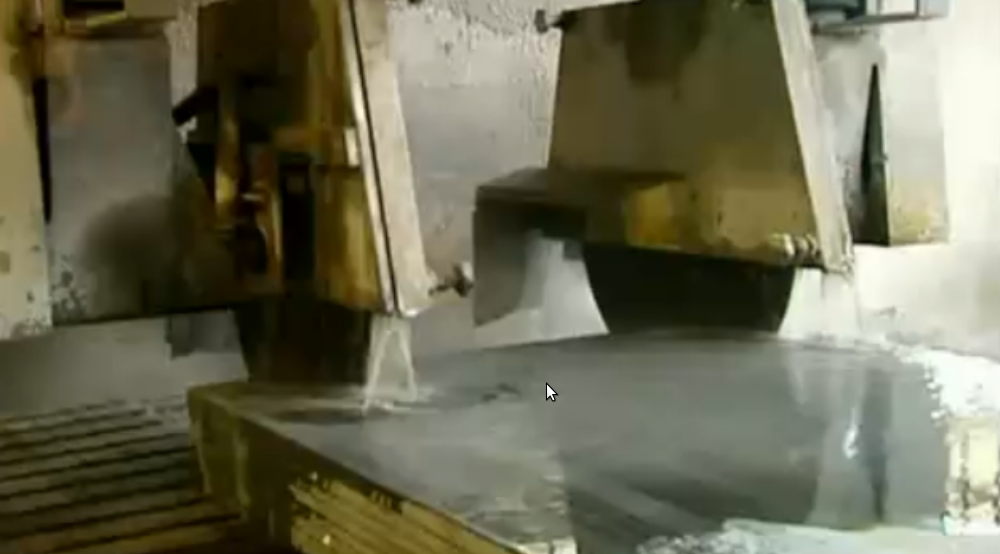
\includegraphics[width=0.4\textwidth]{Pantallazo-6.png}
		        \\ \small {Radial encargada de cortar la pizarra}

	\end{center}

Luego hay que  pulir los bordes con ayuda de una muela de diamante, que deje estos suaves y nivelados.


Una cuarta maquina corta los agujeros por donde salen las bolas para que luego sean lijados a mano.

\begin{center}
	    		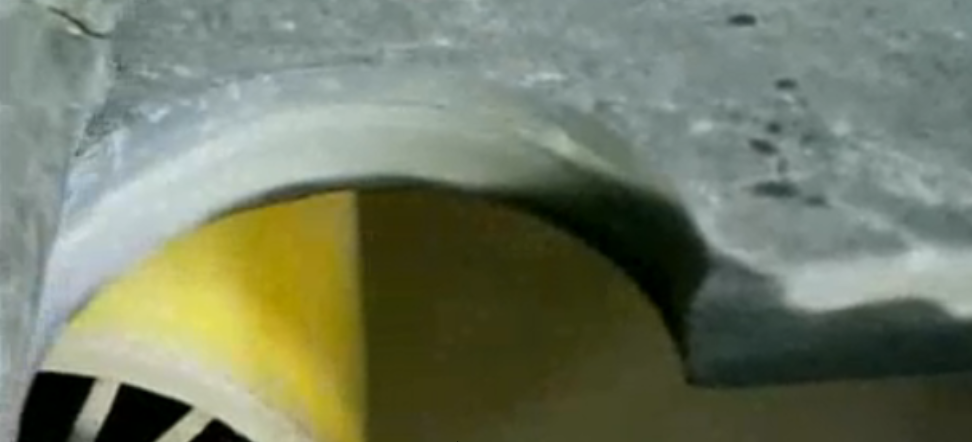
\includegraphics[width=0.4\textwidth]{Pantallazo-7.png}
      \\ \small {Agujeros en la losa de pizarra}


	\end{center}
 Y con esto concluye la preparación del la losa de pizarra.

		\subsubsection {Colocación del paño}
  	
 	Para un perfecto deslizamiento de la bola sobre la losa de pizarra hay que colocar un paño de lana y poliamida azul en nuestro caso. Este deberá ser muy resistente y tener una superficie uniforme para desempeñar correctamente su función.

	La coloración del paño o tapiz se hace de forma totalmente artesanal. Para ello lo colocan primero encima de da losa y entre los agujeros por donde salen las bolas, luego cortan el paño sobrante y finalmente la alisan con un cepillo. 

	\begin{center}
    			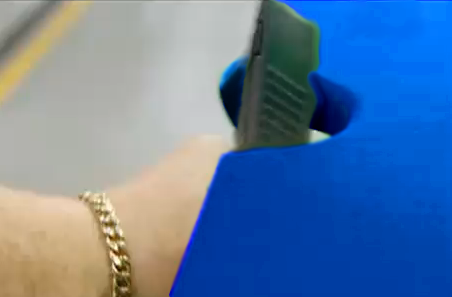
\includegraphics[width=0.4\textwidth]{Pantallazo.png}
			    \\ \small {Colocación del paño o tapete}
		\end{center}
\clearpage
		\subsubsection {Montaje del  borde superior de la mesa de billar}

	En este paso se montará la parte de arriba de la mesa  sin incluir la superficie de juego.

	\begin{center}
    		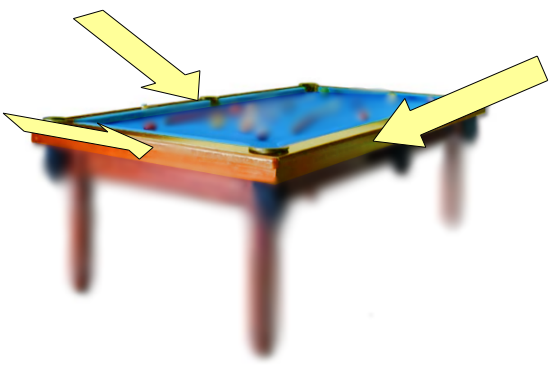
\includegraphics[width=0.4\textwidth]{P1.png}
	\end{center}
	
	Los bordes de la superficie de juego deben tener la elasticidad correcta como para que las bolas reboten sin perder parte de su energía cinética, para ello se hace un compuesto de goma vulcanizada. Este proceso consiste en:
Calentar el caucho crudo en presencia de azufre, con el objetivo de incrementar su dureza y resistencia al frío.

Luego a los bordes se les colocan también unos pliegues de tapetes azules de lana sujetos con unas grapas por la parte interior.


A los bordes interiores se les ancla los bordes exteriores de la mesa de billar, para ello se utiliza cola industrial. La unión de ambos bordes se hace a lo largo de los primeros 2 cm de los bordes de madera. Quedando así 2 cm para la losa de pizarra,  2 cm para el tablón de madera, otros 2 cm para las escuadras de acero. Los bordes exteriores han sido realizados en madera (madera maciza de pino) y encargados en una carpintería industrial, así como las demás piezas de  madera de la mesa.  

\begin{center}
    		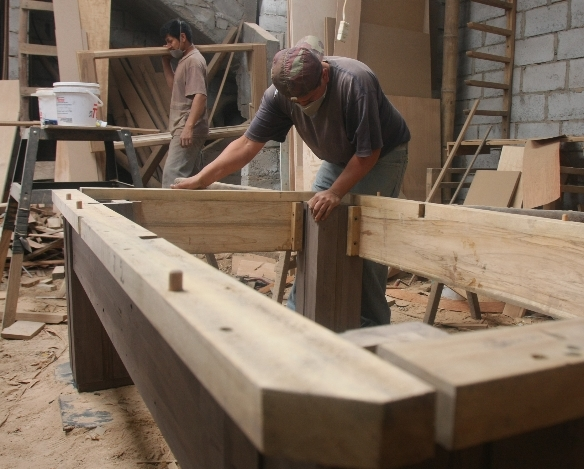
\includegraphics[width=0.4\textwidth]{fc742624-a4ab-44cb-beef-0393ab3abd4a.jpg}
	          \\ \small {Carpinteros realizando partes de una mesa de billar}
	\end{center}



También todas las piezas de madera ha sido pintadas con un barniz para darles un acabado en negro nogal.

El borde de madera consta de 4 piezas de 8 cm de grosor con los agujeros que muestra la figura del apartado 2.2.  Las medidas de estas piezas se pueden ver en esta otra figura:

\begin{center}
    		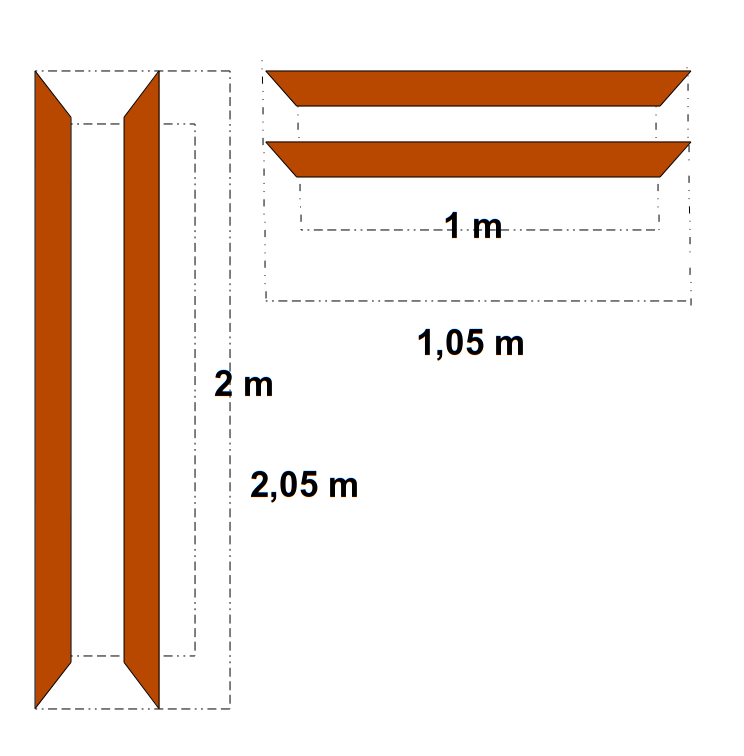
\includegraphics[width=0.4\textwidth]{Exterior.png}
		 \\ \small {Medidas de bordes exteriores}
	\end{center}

Para unir estas cuatro piezas se emplea pegamento industrial (cola especial para madera).
 
Antes de unir el borde interior al borde exterior, en cada agujero de la madera hay que colocar las piezas de plástico duro que revestirán los agujeros y amortiguaran las bolas, ya que en este 
lugar se pretende que las bolas no reboten sino que caigan a las troneras.  Estas piezas van directamente encajadas entre las piezas de madera y goma.  

Para finalizar esta parte se grapan las troneras a esta superficie de madera por la parte de abajo sin que se vean. Las troneras han sido realizadas en terciopelo azul.


\subsubsection {Montaje de la superficie sobre la que irá la losa de pizarra}

\begin{center}
    		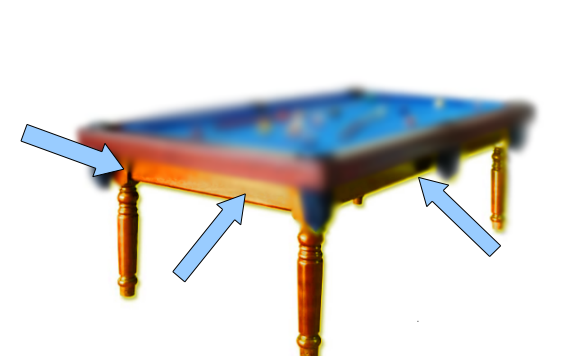
\includegraphics[width=0.5\textwidth]{billar2.png}
	\end{center}


El montaje de esta parte consta de ensamblar nueve piezas de madera, las cuatro patas,  cuatro vigas y un tablón de madera de igual tamaño y forma que la losa de pizarra.
Cuando todas las piezas estén ensambladas, la apariencia será la de una mesa normal, salvo por lo agujeros en el tablón de  madera.

Las vigas tienen 1,5 cm de grosor y las demás medidas las muestra esta figura.

\begin{center}
    		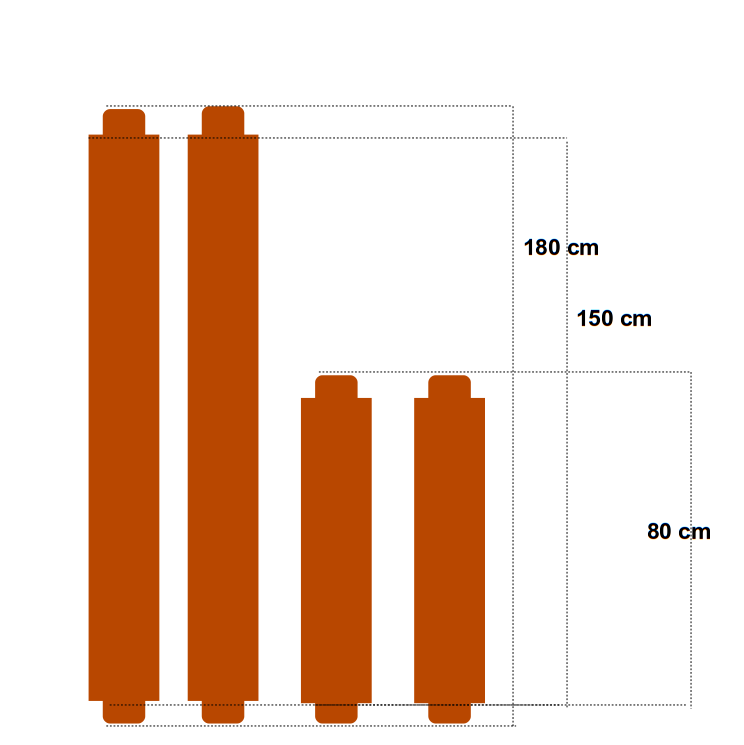
\includegraphics[width=0.5\textwidth]{bigas.png}
		 \\ \small {Medidas de las bigas}
	\end{center}

El ensamblaje se hace con cola industrial y por presión encajando los rebordes de las vigas en las patas (las patas deben llevar una hendidura del tamaño del reborde).
La tabla de madera sí debe ser atornillada a las vigas, con al menos 8 tornillos  (300 mm x 8 mm) para madera a lo largo de la superficie de la mesa,  cerca de la intersección de dos vigas. 
Es muy importante que los tornillos estén bien apretados ya que la losa irá encima y si alguno sobresaliera la superficie del juego podría no quedar recta. 

\begin{center}
    		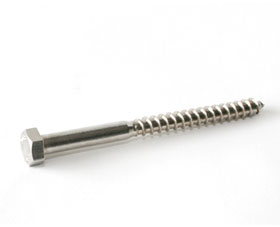
\includegraphics[width=0.25\textwidth]{_42-100.jpg}
		 \\ \small {Tornillos  300 mm x 8 mm}
	\end{center}

\begin{center}

Lo único importante con respecto al diseño de las patas es la medida que se especifica en la figura de abajo y la parte de la pata que irá unida con las vigas. Las medidas deberán corresponderse con las de las vigas mencionadas en otros esquemas.
Además, aunque las patas puedan diferir de la imagen, las cuatro deben ser iguales.   
 		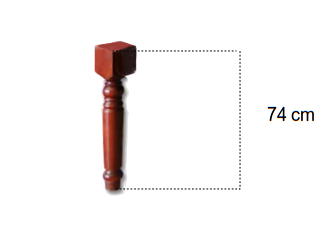
\includegraphics[width=0.5\textwidth]{Pata.png}
		 \\ \small {Dibujo de la pata de la mesa facilitado al carpintero}
	\end{center}


\subsubsection {Unión de las tres partes}

Para unir las tres partes se coloca la losa de pizarra encima de la mesa y se encajan los borde de la mesa. Para la fijación de la tabla de madera con los bordes se emplean pegamento industrial y escuadras de acero, atornilladas con pequeños tornillos de madera.
La colocación de las escuadras  se hace por la parte de debajo de la mesa, donde estas no puedan verse. Se emplearán 8 escuadras. No olvidar sellar también con pegamento industrial. 


\begin{center}
    		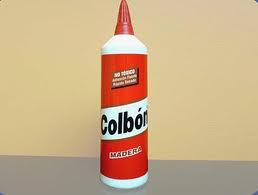
\includegraphics[width=0.3\textwidth]{cola.jpg}
		   \\ \small {Cola especial para madera} \\[0.5cm]
		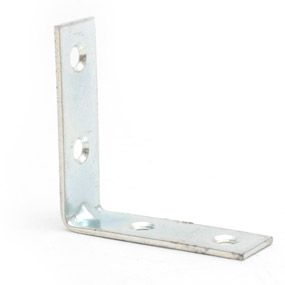
\includegraphics[width=0.25\textwidth]{escuadra.jpg}
		      \\ \small {Ecuadra de acero de 2 cm  x 0,5 cm } 
	\end{center}

\clearpage
\section {Mercado}

El mercado de las mesas de billar suelen abarcarlo en casi su totalidad los locales de ocio, (bares y recreativos...). También hay particulares que desean obtener una
mesa de billar, pero debido a su coste elevado son pocos los que pueden permitirse tener una en sus hogares. 

La mesa de billar descrita en los apartados anteriores está pensada para un uso particular, en casa o centros recreativos privados. Su coste es un tanto elevado, en torno a 2000 \euro.
Algo importante a tener en cuenta antes de adquirir este producto es que para su utilización hay que tener otro tipo de equipación, como son:  bolas, palos, tacos, guantes ... y que el uso adecuado de este producto exige un mantenimiento periódico.  

Este producto se puede encontrar en muchas tiendas de regalos decoración e incluso en alguna tienda de muebles.

En España no hay  mucho consumo de mesas de billar, no obstante se han encontrado algunos sitios para la compra de este producto.
Como son:

\begin{itemize}
  \item http://www.grupobillarcor.es/
 \item http://www.poolspain.com/
 \item http://www.donbillar.com/
 \item http://www.mibillar.com
\end{itemize}
   
Antes se dijo que el consumo en España de mesas de billar no es muy abundantes, esto es si se compara con otros países como Inglaterra o Estados Unidos.

